\documentclass[aspectratio=169,10pt]{beamer}

\usepackage[T1]{fontenc}
\usepackage[utf8]{inputenc}
\usefonttheme{professionalfonts}
\usepackage{amsmath,amssymb,mathtools,bm}
\usepackage{booktabs,tabularx,array,multirow,makecell,colortbl}
\usepackage{graphicx}
\usepackage{tikz}
\usetikzlibrary{arrows.meta,positioning}
\usepackage{ragged2e}
\usepackage{microtype}
\usepackage{appendixnumberbeamer}

\graphicspath{%
  {assets/}%
  {../thesis_phd_math/images/}%
  {../thesis_phd_math/images/ch2/}%
  {../thesis_phd_math/images/ch3/}%
  {../thesis_phd_math/images/ch4/}%
}
% Visual language adapted from the two supplied defense presentations:
% a restrained blue academic layout, a strong title rule, compact footer,
% and contribution ribbons linking results to the specialty passport.

\definecolor{IUBlue}{RGB}{13,88,148}
\definecolor{IUDeepBlue}{RGB}{8,55,101}
\definecolor{IULightBlue}{RGB}{232,242,250}
\definecolor{IUPaleBlue}{RGB}{246,250,253}
\definecolor{GapRed}{RGB}{184,45,54}
\definecolor{GapPale}{RGB}{251,237,239}
\definecolor{ContributionGreen}{RGB}{31,126,93}
\definecolor{ContributionPale}{RGB}{231,246,240}
\definecolor{ConstraintOrange}{RGB}{220,124,32}
\definecolor{ConstraintPale}{RGB}{253,243,230}
\definecolor{Ink}{RGB}{24,31,42}
\definecolor{MidGray}{RGB}{90,99,112}
\definecolor{RuleGray}{RGB}{190,198,207}
\definecolor{SoftGray}{RGB}{244,246,248}

\setbeamercolor{normal text}{fg=Ink,bg=white}
\setbeamercolor{structure}{fg=IUBlue}
\setbeamercolor{frametitle}{fg=Ink,bg=white}
\setbeamercolor{title}{fg=white,bg=IUBlue}
\setbeamercolor{subtitle}{fg=white,bg=IUBlue}
\setbeamercolor{itemize item}{fg=IUBlue}
\setbeamercolor{itemize subitem}{fg=IUBlue}
\setbeamercolor{enumerate item}{fg=white,bg=IUBlue}
\setbeamercolor{block title}{fg=white,bg=IUBlue}
\setbeamercolor{block body}{fg=Ink,bg=IUPaleBlue}
\setbeamercolor{alerted text}{fg=GapRed}
\setbeamercolor{claimbar}{fg=IUDeepBlue,bg=IULightBlue}

\setbeamerfont{title}{size=\Large,series=\bfseries}
\setbeamerfont{subtitle}{size=\normalsize}
\setbeamerfont{frametitle}{size=\Large,series=\mdseries}
\setbeamerfont{footline}{size=\scriptsize}
\setbeamerfont{block title}{series=\bfseries}

\setbeamersize{text margin left=0.55cm,text margin right=0.55cm}
\setbeamertemplate{navigation symbols}{}
\setbeamertemplate{itemize item}{\raise0.15ex\hbox{\color{IUBlue}\small$\bullet$}}
\setbeamertemplate{itemize subitem}{\raise0.12ex\hbox{\color{IUBlue}\scriptsize$\blacktriangleright$}}
\setbeamertemplate{enumerate item}{%
  
\begin{tikzpicture}[baseline=(n.base)]
    \node[circle,fill=IUBlue,inner sep=1.25pt,text=white,font=\bfseries\scriptsize] (n) {\insertenumlabel};
  \end{tikzpicture}%
}

\setbeamertemplate{frametitle}{%
  \nointerlineskip
  \begin{beamercolorbox}[wd=\paperwidth,ht=0.78cm,dp=0.22cm,leftskip=0.55cm,rightskip=0.45cm]{frametitle}%
    \usebeamerfont{frametitle}\insertframetitle
    \hfill
    \raisebox{-0.05ex}{%
      
\begin{tikzpicture}[baseline=(brand.base)]
        \node[draw=IUBlue,line width=0.45pt,inner xsep=4pt,inner ysep=2pt,
          text=IUBlue,font=\bfseries\tiny] (brand) {INNOPOLIS UNIVERSITY};
      \end{tikzpicture}}
  \end{beamercolorbox}%
  \nointerlineskip
  \begin{beamercolorbox}[wd=\paperwidth,ht=0.075cm,dp=0cm]{title rule}\end{beamercolorbox}%
}
\setbeamercolor{title rule}{bg=IUBlue}

\setbeamertemplate{footline}{%
  \leavevmode
  \hbox{%
    \begin{beamercolorbox}[wd=.36\paperwidth,ht=0.30cm,dp=0.13cm,leftskip=0.55cm]{footline}%
      \color{MidGray}\insertshortauthor
    \end{beamercolorbox}%
    \begin{beamercolorbox}[wd=.38\paperwidth,ht=0.30cm,dp=0.13cm,center]{footline}%
      \color{MidGray}Innopolis, 2026
    \end{beamercolorbox}%
    \begin{beamercolorbox}[wd=.26\paperwidth,ht=0.30cm,dp=0.13cm,rightskip=0.55cm plus 1fil]{footline}%
      \color{MidGray}\insertframenumber\,/\,\inserttotalframenumber
    \end{beamercolorbox}%
  }
}

\setbeamertemplate{blocks}[rounded][shadow=false]

\tikzset{
  flowbox/.style={
    draw=IUBlue, line width=0.7pt, rounded corners=2pt,
    fill=IUPaleBlue, align=center, inner sep=4pt,
    minimum height=0.75cm, font=\small
  },
  contribution/.style={
    draw=ContributionGreen, line width=0.8pt, rounded corners=2pt,
    fill=ContributionPale, align=center, inner sep=4pt,
    minimum height=0.78cm, font=\small
  },
  gapbox/.style={
    draw=GapRed, line width=0.8pt, rounded corners=2pt,
    fill=GapPale, align=center, inner sep=4pt,
    minimum height=0.78cm, font=\small
  },
  constraintbox/.style={
    draw=ConstraintOrange, line width=0.8pt, rounded corners=2pt,
    fill=ConstraintPale, align=center, inner sep=4pt,
    minimum height=0.78cm, font=\small
  },
  processarrow/.style={-{Latex[length=2.0mm,width=1.4mm]},line width=0.8pt,draw=IUBlue},
  rejectarrow/.style={-{Latex[length=1.9mm,width=1.35mm]},line width=0.7pt,draw=GapRed,dashed},
  tinylabel/.style={font=\scriptsize,text=MidGray,align=center}
}

\newcommand{\source}[1]{%
  \par\vspace{0.8mm}{\color{MidGray}\scriptsize Source: #1\par}%
}

\newcommand{\claimbar}[2]{%
  \vfill
  \begin{beamercolorbox}[wd=\textwidth,sep=2.0pt,left]{claimbar}%
    \fontsize{5.9}{6.8}\selectfont
    \parbox[t]{0.755\textwidth}{\raggedright\textbf{#1}}\hfill%
    \parbox[t]{0.205\textwidth}{\raggedleft #2}
  \end{beamercolorbox}%
}

\newcommand{\metriccard}[3][IUBlue]{%
  \begin{tikzpicture}[baseline=(m.base)]
    \node[draw=#1,line width=0.65pt,rounded corners=2pt,fill=#1!7,
      text width=2.75cm,minimum height=1.25cm,align=center,inner sep=3pt] (m) {%
      {\color{#1}\bfseries\Large #2}\\[-0.2ex]
      {\footnotesize #3}};
  \end{tikzpicture}%
}

\newcommand{\smalltag}[2][IUBlue]{%
  \tikz[baseline=(t.base)]\node[draw=#1,rounded corners=1.5pt,fill=#1!7,
    text=#1,inner xsep=3pt,inner ysep=1.5pt,font=\bfseries\footnotesize] (t) {#2};%
}

\newcommand{\takeaway}[1]{%
  \begin{beamercolorbox}[wd=\textwidth,sep=4pt,left]{claimbar}%
    \small\textbf{Takeaway:} #1
  \end{beamercolorbox}%
}


\title[Mathematical modeling and motion planning]{%
  Mathematical Modeling and Motion Planning\\
  for Robotic Manipulation of Deformable Linear Objects}
\author[Karam Almaghout]{Karam Almaghout}
\institute{Innopolis University}
\date{Innopolis, 2026}

\hypersetup{
  pdftitle={Mathematical Modeling and Motion Planning for Robotic Manipulation of Deformable Linear Objects},
  pdfauthor={Karam Almaghout},
  colorlinks=true,
  linkcolor=IUBlue,
  urlcolor=IUBlue
}

\newcommand{\R}{\mathbb{R}}
\newcommand{\Cfree}{\mathcal C_{\mathrm{free}}}
\definecolor{GoalPurple}{RGB}{108,76,178}
\newcolumntype{Y}{>{\RaggedRight\arraybackslash}X}
\newcolumntype{C}[1]{>{\Centering\arraybackslash}p{#1}}

\begin{document}

% =============================================================================
% 1. Title
% =============================================================================
\begin{frame}[plain]
  \centering
  \vspace*{0.52cm}
  {\color{IUBlue}\rule{\textwidth}{1.0pt}}\par
  \vspace{0.45cm}
  {\usebeamerfont{title}\color{Ink}\inserttitle\par}
  \vspace{0.25cm}
  {\color{IUBlue}\rule{0.28\textwidth}{2.2pt}}\par

  \vspace{0.58cm}
  {\large\bfseries Karam Almaghout\par}
  {\footnotesize\color{MidGray}Candidate\par}

  \vspace{0.24cm}
  {\small\textbf{Scientific supervisor:} Alexandr Klimchik, PhD\par}
  {\small Innopolis University\par}

  \vspace{0.24cm}
  {\footnotesize\textbf{Specialty 1.2.2}\par}
  {\footnotesize Mathematical modeling, numerical methods and software packages\par}

  \vfill
  {\small\color{MidGray}Thesis for the degree of Candidate of Technical Sciences\par}
\end{frame}

% =============================================================================
% 2. Research problem
% =============================================================================
\begin{frame}[t]{Relevance and research problem}
  \begin{columns}[T,onlytextwidth]
    \begin{column}{0.42\textwidth}
      \centering
      \includegraphics[width=0.93\linewidth,height=2.20cm,keepaspectratio]{Testing-board.jpg}\\[-0.2ex]
      {\footnotesize Wire-harness assembly}

      \vspace{0.18cm}
      \includegraphics[width=0.93\linewidth,height=2.08cm,keepaspectratio]{threads.png}\\[-0.2ex]
      {\footnotesize Surgical-thread manipulation}
    \end{column}

    \begin{column}{0.56\textwidth}
      \small
      A \textbf{deformable linear object (DLO)} is a cable, wire, rope,
      hose, or thread whose complete shape changes during manipulation.

      \vspace{0.20cm}
      \begin{itemize}
        \item Distributed compliance makes the cable shape high-dimensional;
          the two endpoints do not determine it.
        \item Material and dynamic parameters are difficult to identify for
          each object.
        \item Local shape controllers may fail for large transformations,
          including a reversal of concavity.
        \item Collision-free endpoint paths or static cable shapes do not
          guarantee collision-free motion of every cable segment.
      \end{itemize}

      \vspace{0.10cm}
      \textbf{Research problem.} Control and route a planar DLO
      with two robots using its geometry, without prior identification of
      cable parameters (bending, stiffness, ..).
    \end{column}
  \end{columns}
  % \source{Dissertation, Introduction and Chapter 1.}
\end{frame}

% =============================================================================
% 3. Goal and objectives
% =============================================================================
\begin{frame}[t]{Goal and research objectives}
  \begin{columns}[T,onlytextwidth]
    \begin{column}{0.30\textwidth}
      \centering
      \includegraphics[width=\linewidth,height=2.35cm,keepaspectratio]{conc_1inter_c.png}\\[-0.2ex]
      {\scriptsize Large shape deformation}

      \vspace{0.30cm}
      
\includegraphics[width=\linewidth,height=2.35cm,keepaspectratio]{gcr_problem.png}\\[-0.2ex]
      {\scriptsize Routing among obstacles}
    \end{column}

    \begin{column}{0.68\textwidth}
      \footnotesize
      \textbf{Goal.} Develop mathematical models and effective numerical
      methods for dual-arm shape control and routing of DLOs under large planar
      deformations and workspace obstacles, without prior identification of
      dynamic or material parameters.

      \vspace{0.16cm}
      \textbf{Research objectives}
      \begin{enumerate}
        \item Reconstruct and track a marker-free planar cable from images.
        \item Generate length-feasible intermediary configurations, including
          opposite-concavity transformations.
        \item Model local robot--cable kinematics and calculate bounded
          dual-arm motion.
        \item Plan a cable route among static obstacles with valid
          swept motion and endpoint correspondence.
        \item Implement and verify the developed models and numerical methods.
      \end{enumerate}

      \vspace{0.02cm}
    \end{column}
  \end{columns}
  % \source{Dissertation, Introduction: goal, object, subject, and objectives.}
\end{frame}

% =============================================================================
% 4. Formal problem setup
% =============================================================================
\begin{frame}[t]{Problem formulation and setup}
  \footnotesize
  The cable centerline is represented by ordered points
  \(
    \bm p=[\bm p_1,\ldots,\bm p_N]^{\mathsf T}\in\R^{2N}
  \), with nominal segment length \(l_s\).

  \vspace{0.20cm}
  \renewcommand{\arraystretch}{1.32}
  \setlength{\tabcolsep}{4pt}
  \begin{tabularx}{\textwidth}{>{\bfseries}p{2.00cm}YYY}
    \toprule
    \tablehead{Problem} & \tablehead{Given} & \tablehead{Required} &
      \tablehead{Validity conditions}\\
    \midrule
    Shape control &
      Current shape \(\bm p\), target \(\bm t\), and two end-effector poses
      \(\bm r\). &
      Reference profiles \(\bm p^0,\ldots,\bm p^K=\bm t\) and bounded
      end-effector velocities \(\dot{\bm r}\). &
      Approximately fixed discrete length, bounded robot velocities, and
      minimization of aggregate shape error.\\
    \addlinespace[0.10cm]
    Global routing &
      Ordered start and goal configurations \(C_{\mathrm s},C_{\mathrm g}\)
      and known static obstacles \(\mathcal O\). &
      A sequence \(\mathcal P=(C_0,\ldots,C_K)\), from start to goal. &
      Every configuration is statically admissible; every neighboring
      transition is collision-free and preserves endpoint correspondence.\\
    \bottomrule
  \end{tabularx}

  \vspace{0.24cm}
  % \textbf{Validation boundary.} Chapter 3 uses image feedback in physical
  % shape-control experiments. Chapter 4 starts from prescribed ordered
  % configurations and known obstacle geometry and is validated computationally
  % and in MuJoCo.
\end{frame}

% =============================================================================
% 5. Contributions
% =============================================================================
\begin{frame}[t]{Scientific contributions}
  \small
  \begin{enumerate}
    \item \textbf{Virtual Feature Points (VFPs):} an ordered, approximately
      equidistant point representation reconstructed from an image of a marker-free cable.

    \item \textbf{Intermediary-shape planning:} The Angular and Linear Interpolation-based Planner (ALI) for large deformation of shape control.

    \item \textbf{Shape control:} a diminishing-rigidity Jacobian and
      constrained optimization for bounded two-arm motion without identified
      stiffness and bending parameters of the cable.

    \item \textbf{Global Cable Routing (GCR):} an ordered configuration-space
      model and numerical method with guided sampling, Artificial Potential
      Field (APF) bias, projected relaxation, and swept-transition validation.

    \item \textbf{Software and verification:} Vision-based cable detection and tracking, MATLAB simulations, a C++ GCR implementation, physical KUKA experiments, and simulation validation (MuJoCo).
  \end{enumerate}
  % \source{Dissertation, Introduction: scientific novelty and main results.}
\end{frame}

% =============================================================================
% 6. VFP slide -- reconstructed from the July 2024 defense
% =============================================================================
\begin{frame}[t]{Virtual Feature Points (VFPs) Algorithm}
  \begin{columns}[T,onlytextwidth]
    \begin{column}{0.53\textwidth}
      \footnotesize
      \begin{enumerate}
        \item Detect the marked tool and identify the starting cable point.
        \item Segment the marker-free cable using edges and morphology.
        \item Apply Guo--Hall thinning to extract a one-pixel centerline.
        \item Place the center of a circular mask on the starting point.
        \item Record the forward intersection of the mask and centerline as a
          new feature point.
        \item Slide the mask to the new feature point.
        \item Repeat Steps 5 and 6 until the cable end is reached.
      \end{enumerate}
			\small
  \observation{VFPs reconstruct an ordered, approximately equidistant cable
  state from one top-view camera image.}
			\vspace{0.03cm}
			\[
	  \bm p=[\bm p_1,\ldots,\bm p_N]^{\mathsf T},
    \qquad \|\bm p_{n+1}-\bm p_n\|\approx l_s .
  	\]
    \end{column}

    \begin{column}{0.45\textwidth}
      \centering
      
\includegraphics[width=\linewidth,height=2.65cm,keepaspectratio]{vfps-steps.png}
      \vspace{0.08cm}

      
\includegraphics[width=\linewidth,height=3.25cm,keepaspectratio]{vfps_pipeline.png}
    \end{column}
  \end{columns}
	
\end{frame}

% =============================================================================
% 7. ALI -- layout and complete content of the July 2024 slide, final equations
% =============================================================================
\begin{frame}[t]{Cable Path Planning for Large Deformation}
  \vspace{0.10cm}
  {\small\color{IUDeepBlue}\textbf{Aim:} Decompose a complex deformation into
  multiple length-feasible stages.}
  \vspace{0.02cm}

  \begin{columns}[T,onlytextwidth]
    \begin{column}{0.45\textwidth}
      \fontsize{7.1}{7.7}\selectfont
      \setlength{\abovedisplayskip}{2pt}
      \setlength{\belowdisplayskip}{2pt}
      \textbf{Angular and Linear Interpolation-based Planner (ALI)}
      \[
        \bm\Delta=\bm t-\bm p^0,\qquad
        \sigma=\arg\max_{n=1,\ldots,N}\|\bm\Delta_n\|,
      \]
      \[
        K=\left\lfloor\frac{\|\bm\Delta_\sigma\|}{\lambda}\right\rfloor+1,
        \qquad \bm\Theta=\bm\theta^t-\bm\theta^p,
      \]
      \[
        \bm\vartheta=\frac{\bm\Theta}{K},
        \qquad \bm\delta_\sigma=\frac{\bm\Delta_\sigma}{K}.
      \]
      For \(\kappa=1,\ldots,K-1\):
      \[
        \bm p_\sigma^\kappa=\bm p_\sigma^{\kappa-1}+\bm\delta_\sigma,
        \qquad
        \theta_n^\kappa=\theta_n^p+\kappa\vartheta_n,
      \]
      \[
        \bm p_n^\kappa=
        \begin{cases}
        \bm p_{n-1}^\kappa+l_s
          \begin{bmatrix}\cos\theta_n^\kappa\\ \sin\theta_n^\kappa\end{bmatrix},
          & n>\sigma,\\[2.0ex]
        \bm p_{n+1}^\kappa-l_s
          \begin{bmatrix}\cos\theta_n^\kappa\\ \sin\theta_n^\kappa\end{bmatrix},
          & n<\sigma,
        \end{cases}
      \]
      \hfill
			\\
			Final profile: \(\bm p^K=\bm t\).\par
      \vspace{0.02cm}
      {\fontsize{6.3}{6.9}\selectfont
      \(\bm p^0,\bm t\): initial and target profiles;
      \(\sigma\): maximally displaced point; \\ \(\lambda\): maximum reference
      step; \(K\): number of stages; \(l_s\): nominal segment length.}
    \end{column}

    \begin{column}{0.65\textwidth}
      \centering
      \setlength{\tabcolsep}{2pt}
      \begin{tabular}{@{}ccc@{}}
        % \includegraphics[width=0.4\textwidth,height=2.34cm,keepaspectratio]{preliminaries1.png} &
        \includegraphics[width=0.3\textwidth,height=2.34cm,keepaspectratio]{CEP_angles.drawio.png} &
        
\includegraphics[width=0.5\textwidth,height=2.34cm,keepaspectratio]{ali_geometry.png}\\[-0.3ex]
        % \multicolumn{1}{c}{\scriptsize Initial \(\bm p^0\), target \(\bm t\)} &
        \multicolumn{1}{c}{\scriptsize Segment angles} &
        \multicolumn{1}{c}{\scriptsize ALI profiles}
      \end{tabular}

      \vspace{0.06cm}
      \begin{tabular}{@{}cc@{}}
        
\includegraphics[width=0.4\textwidth,height=2.40cm,keepaspectratio]{linear_interpolation.png} &
        
\includegraphics[width=0.4\textwidth,height=2.40cm,keepaspectratio]{ali_interpolation.png}\\[-0.2ex]
        \scriptsize Pointwise linear interpolation & \scriptsize ALI
      \end{tabular}
    \end{column}
  \end{columns}
\end{frame}

% =============================================================================
% 8. Motion planning -- old three-part layout, final dissertation Jacobian
% =============================================================================
\begin{frame}[t]{Motion Planning}
  \vspace{0.10cm}
  {\small\color{IUDeepBlue}\textbf{Aim:} Control the robots' end effectors to
  follow each intermediary shape.}
  \vspace{0.04cm}

  \begin{columns}[T,onlytextwidth]
    \begin{column}{0.31\textwidth}
      \fontsize{7.4}{8.3}\selectfont
      \setlength{\abovedisplayskip}{3pt}
      \setlength{\belowdisplayskip}{3pt}
      \textbf{Constrained shape control}
      \[
        \text{for }\kappa=1,\ldots,K:\quad \quad \quad
      \]
      \[
        \min_{\bm r} \sum_{n=1}^{N}\|\bm p_n^\kappa-\bm p_n\|,
      \]
      \[
        \text{s.t. } \quad 
        \dot{\bm p}=\bm J\dot{\bm r},
        \quad |\dot{\bm r}|\leq\bm\nu 
      \]
			
      \vspace{0.08cm}
      % The point blocks are assembled as
      % \[
      %   m(n)=\arg\min_{m\in\{1,2\}}D_n^m,
      % \]
      \[
        \bm J_{2N \times 6}=\operatorname{blkdiag}(\bm J^1,\bm J^2)
        % \qquad \dot{\bm p}=\bm J\dot{\bm r}.
      \]
      {\scriptsize Points are assigned to the closest endpoints based on nominal cable-order distance.\\
			 \(\bm\nu\) the end-effectors velocities limits.}
    \end{column}

    \begin{column}{0.39\textwidth}
      \fontsize{7.4}{8.3}\selectfont
      \setlength{\abovedisplayskip}{3pt}
      \setlength{\belowdisplayskip}{3pt}
      \textbf{Diminishing-rigidity Jacobian}
      \[
        D_n^m=\eta_n^m l_s,
        \qquad
        d_n^m=\left\|\bm p_n-
        \begin{bmatrix}r_{mx}\\r_{my}\end{bmatrix}\right\|,
      \]
      \[
        \mu_n^m=e^{-|D_n^m-d_n^m|},
      \]
      \[
        \bm J_n^m=\mu_n^m
        \begin{bmatrix}
          1&0&-D_n^m\sin\theta_m\\
          0&1&D_n^m\cos\theta_m
        \end{bmatrix}.
      \]
      \vspace{0.08cm}
      {\scriptsize
			
			\(m\): end effector with pose
      \(\bm r_m=[r_{mx},r_{my},\theta_m]^{\mathsf T}\)\\
      \(\eta_n^m\): number of nominal segments from \(m\) to \(n\)\\
			\(D_n^m\): fully stretched distance, \(d_n^m\): current distance}
    \end{column}

    \begin{column}{0.26\textwidth}
      \centering
      
\includegraphics[width=0.65\linewidth,height=3.52cm,keepaspectratio]{rigidity_geometry.png}

      \vspace{0.12cm}
      \scriptsize
     \(d_n^m\approx D_n^m\), strong coupling.\\[0.10cm]
     \(d_n^m<D_n^m\), diminishing coupling.
    \end{column}
  \end{columns}

  % \observation{The controller uses observed geometry and robot poses; it does
  % not require identified cable parameters.}
\end{frame}

% =============================================================================
% 9. Shape-control evidence summary
% =============================================================================
\begin{frame}[t]{Shape-control results}
	\textbf{Simulation Results} \par
	\scriptsize
	\begin{enumerate}
		\item The cable is modeled as mass-spring model with rigid endpoint grasps.
		\item Two different models are used.
		\item Each model is tested for N = 8, 10, 12, 14
		\item  \(\lambda\) tested from 1 to 100 mm
	\end{enumerate}
	
  \centering
  {\scriptsize\textit{Initial, desired, and ALI profiles}\par}
  \vspace{0.04cm}
  \setlength{\tabcolsep}{2pt}
  \begin{tabular}{@{}cccc@{}}
    \includegraphics[width=0.225\textwidth,height=1.85cm,keepaspectratio]{c1.png} &
    \includegraphics[width=0.225\textwidth,height=1.85cm,keepaspectratio]{c2.png} &
    \includegraphics[width=0.225\textwidth,height=1.85cm,keepaspectratio]{c3.png} &
    \includegraphics[width=0.225\textwidth,height=1.85cm,keepaspectratio]{c4.png}\\[-0.28ex]
  \end{tabular}

  \vspace{0.06cm}
  {\scriptsize\textit{Final simulation results; mean error for \(N=10\)}\par}
  \vspace{0.04cm}
  \begin{tabular}{@{}cccc@{}}
    \includegraphics[width=0.225\textwidth,height=1.85cm,keepaspectratio]{f1_07.png} &
    \includegraphics[width=0.225\textwidth,height=1.85cm,keepaspectratio]{f2_07.png} &
    \includegraphics[width=0.225\textwidth,height=1.85cm,keepaspectratio]{f3_07.png} &
    \includegraphics[width=0.225\textwidth,height=1.85cm,keepaspectratio]{f4_07.png}\\[-0.28ex]
    \scriptsize U: 4.2 mm &
    \scriptsize L: 6.9 mm &
    \scriptsize S: 6.5 mm &
    \scriptsize M: 4.2 mm
  \end{tabular}

\end{frame}

% =============================================================================
% 10. Physical shape-control evidence
% =============================================================================
\begin{frame}[t]{Shape-control results}
  \begin{columns}[T,onlytextwidth]
    \begin{column}{0.5\textwidth}
      \scriptsize
      \textbf{Physical study:} 
			\begin{enumerate}
				\item The cable is a 350 mm long, 9 mm diameter, flexible wire.
				\item The robots are two KUKA LBR iiwa 7 R800 manipulators.
				\item The camera is a top-view RealSense D435.
				\item The number of VFPs is \(N=10\).
				\item The maximum reference step is \(\lambda=10\) mm.
				\item All U/L/S/M and opposite-concavity tasks were achieved.
			\end{enumerate}
			\end{column}
			\begin{column}{0.5\textwidth}
				\centering
      
\includegraphics[width=\linewidth,height=2.15cm,keepaspectratio]{kuka_setup.jpg}
			\end{column}
  \end{columns}

  \centering
  % {\scriptsize\textit{U/L/S/M shapes: initial and intermediary profiles (top), final result (bottom)}\par}
  \vspace{0.08cm}
  \setlength{\tabcolsep}{1.5pt}
  \begin{tabular}{@{}>{\centering\arraybackslash}m{2.0cm}
    *{4}{>{\centering\arraybackslash}m{0.123\textwidth}}@{}}
			\scriptsize\makecell[c]{Initial, desired,\\and ALI profiles}&
    \includegraphics[width=0.2\textwidth,height=0.70cm,keepaspectratio]{U1inter_c.png} &
    \includegraphics[width=0.2\textwidth,height=0.70cm,keepaspectratio]{L1inter_c.png} &
    \includegraphics[width=0.2\textwidth,height=0.70cm,keepaspectratio]{S1inter_c.png} &
    \includegraphics[width=0.2\textwidth,height=0.70cm,keepaspectratio]{M1inter_c.png}\\[-0.32ex]
			\scriptsize\makecell[c]{Final results,\\mean error}&
			\includegraphics[width=0.2\textwidth,height=0.70cm,keepaspectratio]{U1f_c.png} &
    \includegraphics[width=0.2\textwidth,height=0.70cm,keepaspectratio]{L1f_c.png} &
    \includegraphics[width=0.2\textwidth,height=0.70cm,keepaspectratio]{S1f_c.png} &
    \includegraphics[width=0.2\textwidth,height=0.70cm,keepaspectratio]{M1f_c.png}\\[-1.32ex]
		&
    \scriptsize U: 11.7 mm & \scriptsize L: 10.9 mm &
    \scriptsize S: 10.6 mm & \scriptsize M: 5.2 mm
  \end{tabular}

  % {\scriptsize\textit{Opposite-concavity shapes: initial and intermediary profiles (top), final result (bottom)}\par}
  \vspace{0.12cm}
  \begin{tabular}{@{}>{\centering\arraybackslash}m{2.0cm}
    *{4}{>{\centering\arraybackslash}m{0.123\textwidth}}@{}}
			\scriptsize\makecell[c]{Initial, desired,\\and ALI profiles}&
    \includegraphics[width=0.2\textwidth,height=0.70cm,keepaspectratio]{conc_1inter_c.png} &
    \includegraphics[width=0.2\textwidth,height=0.70cm,keepaspectratio]{conc_2inter_c.png} &
    \includegraphics[width=0.2\textwidth,height=0.70cm,keepaspectratio]{conc_3inter_c.png} &
    \includegraphics[width=0.2\textwidth,height=0.70cm,keepaspectratio]{conc_4inter_c.png}\\[-0.32ex]
			\scriptsize\makecell[c]{Final results,\\mean error}&
    \includegraphics[width=0.2\textwidth,height=0.70cm,keepaspectratio]{conc_1f_c.png} &
    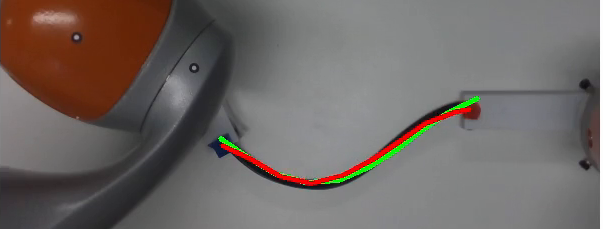
\includegraphics[width=0.2\textwidth,height=0.70cm,keepaspectratio]{conc_2f_c.png} &
    \includegraphics[width=0.2\textwidth,height=0.70cm,keepaspectratio]{conc_3f_c.png} &
    \includegraphics[width=0.2\textwidth,height=0.70cm,keepaspectratio]{conc_4f_c.png}\\[-1.32ex]
    &
		\scriptsize sce.1: 12.4 mm & \scriptsize sce.2: 9.0 mm &
    \scriptsize sce.3: 8.1 mm & \scriptsize sce.4: 4.5 mm
  \end{tabular}
\end{frame}

% =============================================================================
% 11. Bidirectional search structure
% =============================================================================
\begin{frame}[t]{Global Cable Routing (1/3): bi-tree planning structure}
  \begin{columns}[T,onlytextwidth]
    \begin{column}{0.52\textwidth}
      \centering
      
\includegraphics[width=\linewidth,height=3.55cm,keepaspectratio]{gcr_problem.png}
      \vspace{0.03cm}

      {\footnotesize
      \[
        C=(p_1,\ldots,p_N)\in\R^{2N},\qquad
        \mathcal P=(C_0,\ldots,C_K).
      \]
      \textbf{Each vertex is a complete ordered cable configuration.}}
    \end{column}

    \begin{column}{0.46\textwidth}
      \centering
      {\footnotesize\color{IUDeepBlue}\textbf{Two trees grow toward one another}\par}
      \vspace{0.08cm}
      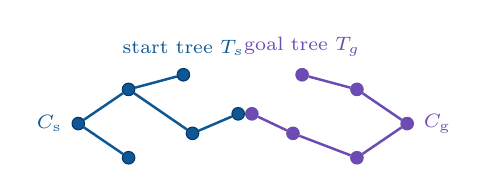
\begin{tikzpicture}[
        x=0.58cm,y=0.62cm,
        every node/.style={font=\scriptsize},
        sNode/.style={circle,fill=IUBlue,draw=IUDeepBlue,inner sep=1.6pt},
        gNode/.style={circle,fill=GoalPurple,draw=GoalPurple,inner sep=1.6pt},
        sEdge/.style={draw=IUBlue,line width=0.9pt},
        gEdge/.style={draw=GoalPurple,line width=0.9pt}]
        \node[sNode,label=left:{\color{IUBlue}\(C_{\mathrm s}\)}] (s0) at (0,1.7) {};
        \node[sNode] (s1) at (1.1,2.4) {};
        \node[sNode] (s2) at (1.1,1.0) {};
        \node[sNode] (s3) at (2.3,2.7) {};
        \node[sNode] (s4) at (2.5,1.5) {};
        \node[sNode] (s5) at (3.5,1.9) {};
        \draw[sEdge] (s0)--(s1) (s0)--(s2) (s1)--(s3) (s1)--(s4) (s4)--(s5);
        \node[gNode,label=right:{\color{GoalPurple}\(C_{\mathrm g}\)}] (g0) at (7.2,1.7) {};
        \node[gNode] (g1) at (6.1,2.4) {};
        \node[gNode] (g2) at (6.1,1.0) {};
        \node[gNode] (g3) at (4.9,2.7) {};
        \node[gNode] (g4) at (4.7,1.5) {};
        \node[gNode] (g5) at (3.8,1.9) {};
        \draw[gEdge] (g0)--(g1) (g0)--(g2) (g1)--(g3) (g2)--(g4) (g4)--(g5);
        % \draw[-{Latex[length=2mm]},dashed,thick,draw=MidGray] (s5)--(g5);
        \node[above=0.03cm of s3,text=IUBlue] {start tree \(T_s\)};
        \node[above=0.03cm of g3,text=GoalPurple] {goal tree \(T_g\)};
      \end{tikzpicture}

      {\fontsize{7.4}{8.2}\selectfont
      \[
        T_s=(V_s,E_s),\quad V_s=\{C_{\mathrm s}\},\quad E_s=\emptyset,
      \]
      \[
        T_g=(V_g,E_g),\quad V_g=\{C_{\mathrm g}\},\quad E_g=\emptyset.
      \]
      \textbf{Alternate the roles every iteration:}
      \[
      (T_{\mathrm{act}},T_{\mathrm{opp}})=
      \begin{cases}
        (T_s,T_g),&i\ \text{odd},\\
        (T_g,T_s),&i\ \text{even}.
      \end{cases}
      \]}
    \end{column}
  \end{columns}

  \vspace{0.06cm}
  \centering
  {\scriptsize\color{IUDeepBlue}\textbf{Planner loop:}\enspace
  initialize \(T_s,T_g\) \(\rightarrow\) alternate active tree
  \(\rightarrow\) expand \(\rightarrow\) try the opposite tree
  \(\rightarrow\) trace and shortcut the connected path.\par}
\end{frame}

% =============================================================================
% 12. One alternating tree expansion
% =============================================================================
\begin{frame}[t]{Global Cable Routing (2/3): one tree-expansion step}
  \begin{beamercolorbox}[wd=\textwidth,center]{normal text}
  \footnotesize
  Expand \({\color{IUBlue}T_{\mathrm{act}}}\) toward a target in
  \({\color{GoalPurple}T_{\mathrm{opp}}}\); then exchange the tree roles.
  \end{beamercolorbox}
  \vspace{0.01cm}
  \setlength{\abovedisplayskip}{2pt}
  \setlength{\belowdisplayskip}{2pt}

  \begin{columns}[T,onlytextwidth]
    \begin{column}{0.315\textwidth}
      \centering
      {\footnotesize\color{IUDeepBlue}\textbf{1. Generate candidate}\par}
      
\includegraphics[width=\linewidth,height=1.70cm,keepaspectratio]{gcr_raw.pdf}
      {\fontsize{6.9}{7.7}\selectfont
      \[
      C^{\mathrm{raw}}\sim
      \begin{cases}
        \text{goal biased},&p_g,\\
        \text{tree biased},&p_t,\\
        \text{broad random},&1-p_g-p_t.
      \end{cases}
      \]}
    \end{column}

    \begin{column}{0.315\textwidth}
      \centering
      {\footnotesize\color{IUDeepBlue}\textbf{2. Bias toward \(T_{\mathrm{opp}}\)}\par}
      
\includegraphics[width=\linewidth,height=1.70cm,keepaspectratio]{gcr_apf.pdf}
      {\fontsize{6.9}{7.7}\selectfont
      \makebox[\linewidth][c]{Target: \(C^{\mathrm{target}}\in V_{\mathrm{opp}}\).}
      \[
        U=U_{\mathrm{att}}(C,C^{\mathrm{target}})+U_{\mathrm{rep}}(C,\mathcal O),
      \]
      \[
        C^b=C^{\mathrm{raw}}-\eta\nabla U(C^{\mathrm{raw}}).
      \]}
    \end{column}

    \begin{column}{0.315\textwidth}
      \centering
      {\footnotesize\color{IUDeepBlue}\textbf{3. Relax about \(T_{\mathrm{act}}\)}\par}
      
\includegraphics[width=\linewidth,height=1.70cm,keepaspectratio]{gcr_relax.pdf}
      {\fontsize{6.9}{7.7}\selectfont
      \[
        C^{\mathrm{ref}}=\arg\min_{C_i\in V_{\mathrm{act}}}d(C_i,C^b),
      \]
      \[
        C^{\mathrm{relax}}=\operatorname{Relax}(C^b,C^{\mathrm{ref}},\mathcal O).
      \]
      {\scriptsize Accept only if \(C^{\mathrm{relax}}\in\Cfree\); otherwise reject.}}
    \end{column}
  \end{columns}

  \vspace{0.01cm}
  \centering
  {\scriptsize\color{IUDeepBlue}\textbf{4. Choose an ordered parent and insert}\par}
  {\fontsize{6.7}{7.5}\selectfont
  \[
  \begin{aligned}
    \mathcal V_{\mathrm{par}}=
    \bigl\{(C_i,\sigma):\;&C_i\in V_{\mathrm{act}},\ \sigma\in\{+1,-1\},\\[-0.2ex]
    &d(C_i,(C^{\mathrm{relax}})^\sigma)\leq\epsilon,\quad
    \Gamma(C_i,(C^{\mathrm{relax}})^\sigma)=1\bigr\}.
  \end{aligned}
  \]
  If \(\mathcal V_{\mathrm{par}}=\emptyset\), reject. Otherwise choose
  \(C^{\mathrm{par}}\), set \(C^{\mathrm{new}}=(C^{\mathrm{relax}})^{\sigma^*}\),
  and insert \((C^{\mathrm{par}},C^{\mathrm{new}})\) into \(T_{\mathrm{act}}\).\par}
\end{frame}

% =============================================================================
% 13. Validate and connect the two trees
% =============================================================================
\begin{frame}[t]{Global Cable Routing (3/3): validate, connect, and refine}
  \centering
  {\scriptsize\color{IUDeepBlue}
  \(C^{\mathrm{new}}\in T_{\mathrm{act}}\)
  \(\rightarrow\)
  \(\mathcal V_{\mathrm{conn}}=\operatorname{Near}(T_{\mathrm{opp}},C^{\mathrm{new}},\epsilon)\)
  \(\rightarrow\) filter by \(\Gamma\) in start-to-goal order
  \(\rightarrow\) connect \(T_s\) and \(T_g\).\par}

  \vspace{0.04cm}
  \begin{columns}[T,onlytextwidth]
    \begin{column}{0.60\textwidth}
      \centering
      \setlength{\tabcolsep}{2pt}
      \begin{tabular}{@{}cc@{}}
        
\includegraphics[width=0.28\textwidth,height=1.90cm,keepaspectratio]{transition_free.pdf} &
        
\includegraphics[width=0.28\textwidth,height=1.90cm,keepaspectratio]{transition_blocked.pdf}\\[-0.25ex]
        \scriptsize Accepted bridge & \scriptsize Rejected bridge
      \end{tabular}

      \vspace{0.04cm}
      {\fontsize{6.8}{7.6}\selectfont
      \[
        \mathcal S_k(C^a,C^b)=\operatorname{conv}
        \{p_k^a,p_{k+1}^a,p_{k+1}^b,p_k^b\},\qquad
        \mathcal S_k\cap\mathcal O=\emptyset\ \ \forall k.
      \]
      \[
        u(C)=\frac{p_N-p_1}{\|p_N-p_1\|},\qquad
        u(C^a)^{\mathsf T}u(C^b)\geq\cos\theta_{\max}.
      \]
      \[
        \Gamma=\operatorname{PathFree}\land\operatorname{AxisConsistent}
        \land\operatorname{EndpointFeasible}.
      \]}
    \end{column}

    \begin{column}{0.38\textwidth}
      \footnotesize
      \textbf{After inserting \(C^{\mathrm{new}}\):}
      \begin{enumerate}
        \item find nearby vertices in \(T_{\mathrm{opp}}\);
        \item accept a bridge only if \(\Gamma=1\);
        \item trace both parent chains and concatenate them from start to goal;
        \item shortcut the route using the same \(\Gamma\) test.
      \end{enumerate}

      \vspace{0.06cm}
      {\scriptsize\color{MidGray}
      The predicate \(\Gamma\) is used for parent insertion, inter-tree
      connection, and shortcut edges.}
    \end{column}
  \end{columns}

  \vspace{0.04cm}
  {\scriptsize\color{IUDeepBlue}\textbf{Result:}\enspace
  \(T_s\leftrightarrow T_g\Rightarrow\mathcal P_{\mathrm{raw}}
  \Rightarrow\mathcal P_{\mathrm{ref}}\), with
  \(\Gamma(C_i,C_{i+1})=1\) for every retained edge.\par}
\end{frame}

% =============================================================================
% 13. GCR computational evidence
% =============================================================================
\begin{frame}[t]{Global Cable Routing: computational results}
  \begin{columns}[T,onlytextwidth]
    \begin{column}{0.64\textwidth}
      \centering
      \setlength{\tabcolsep}{3pt}
      \begin{tabular}{@{}cc@{}}
        
\includegraphics[width=0.29\textwidth,height=2.00cm,keepaspectratio]{route_arc.pdf} &
        
\includegraphics[width=0.29\textwidth,height=2.00cm,keepaspectratio]{route_gate.pdf}\\[-0.2ex]
        \scriptsize Arc to straight & \scriptsize Narrow gate\\[0.02cm]
        
\includegraphics[width=0.29\textwidth,height=2.00cm,keepaspectratio]{route_trap.pdf} &
        
\includegraphics[width=0.29\textwidth,height=2.00cm,keepaspectratio]{route_corridor.pdf}\\[-0.2ex]
        \scriptsize U-shaped trap & \scriptsize L-corridor
      \end{tabular}
    \end{column}

    \begin{column}{0.34\textwidth}
      \footnotesize
      \renewcommand{\arraystretch}{1.20}
      \setlength{\tabcolsep}{4pt}
      \begin{tabularx}{\linewidth}{>{\bfseries}p{1.75cm}Y}
        \toprule
        Protocol & 10 scenarios, 1000 independent seeds each\\
        \midrule
        Valid routes & 10,000 of 10,000 tested runs\\
        Mean time & \(0.008\pm0.003\) to \(1.306\pm0.871\) s\\
        Raw path & \(13\pm2\) to \(25\pm4\) configurations\\
        Refined path & \(3\pm1\) to \(9\pm1\) configurations\\
        \bottomrule
      \end{tabularx}

      \vspace{0.12cm}
    \end{column}
  \end{columns}

  \observation{All tested paths satisfied the stated static and transition
  predicates. }
\end{frame}

% =============================================================================
% 14. MuJoCo evidence
% =============================================================================
\begin{frame}[t]{Global Cable Routing: MuJoCo validation}
  
  \begin{columns}[T,onlytextwidth]
    \begin{column}{0.71\textwidth}
      \centering
      
\includegraphics[width=0.92\linewidth,height=2.20cm,keepaspectratio]{mujoco_setup.pdf} 
      \vspace{0.3cm}
      \hline
      \vspace{0.3cm}
      \centering
      \setlength{\tabcolsep}{1.5pt}
      \begin{tabular}{@{}c@{\hspace{1mm}}cccc@{}}
        & \scriptsize Start
        & \scriptsize \makecell{Intermediate\\stage 1}
        & \scriptsize \makecell{Intermediate\\stage 2}
        & \scriptsize End\\[0.03cm]
        \scriptsize S1 &
        \includegraphics[width=0.155\textwidth,height=1.48cm,keepaspectratio]{mujoco/scenario_01/start.pdf} &
        \includegraphics[width=0.155\textwidth,height=1.48cm,keepaspectratio]{mujoco/scenario_01/33pct.pdf} &
        \includegraphics[width=0.155\textwidth,height=1.48cm,keepaspectratio]{mujoco/scenario_01/67pct.pdf} &
        \includegraphics[width=0.155\textwidth,height=1.48cm,keepaspectratio]{mujoco/scenario_01/end.pdf}\\[0.08cm]
        \scriptsize S7 &
        \includegraphics[width=0.155\textwidth,height=1.48cm,keepaspectratio]{mujoco/scenario_07/start.pdf} &
        \includegraphics[width=0.155\textwidth,height=1.48cm,keepaspectratio]{mujoco/scenario_07/33pct.pdf} &
        \includegraphics[width=0.155\textwidth,height=1.48cm,keepaspectratio]{mujoco/scenario_07/67pct.pdf} &
        \includegraphics[width=0.155\textwidth,height=1.48cm,keepaspectratio]{mujoco/scenario_07/end.pdf}\\[0.08cm]
        \scriptsize S10 &
        \includegraphics[width=0.155\textwidth,height=1.48cm,keepaspectratio]{mujoco/scenario_10/start.pdf} &
        \includegraphics[width=0.155\textwidth,height=1.48cm,keepaspectratio]{mujoco/scenario_10/33pct.pdf} &
        \includegraphics[width=0.155\textwidth,height=1.48cm,keepaspectratio]{mujoco/scenario_10/67pct.pdf} &
        \includegraphics[width=0.155\textwidth,height=1.48cm,keepaspectratio]{mujoco/scenario_10/end.pdf}
      \end{tabular}
    \end{column}

    \begin{column}{0.27\textwidth}
      \vspace{1.7cm}
      \centering
      \scriptsize
      \renewcommand{\arraystretch}{1.06}
      \begin{tabular}{r@{\hspace{0.30cm}}r@{\hspace{0.30cm}}r}
        \toprule
        Sc. & RMSE & Max.\\
            & [mm] & [mm]\\
        \midrule
        1  & 2.20 & 3.41\\
        2  & 2.22 & 3.72\\
        3  & 4.32 & 6.49\\
        4  & \textbf{1.60} & \textbf{2.31}\\
        5  & 1.87 & 2.70\\
        6  & 2.08 & 3.32\\
        7  & 4.66 & 7.81\\
        8  & 4.13 & 6.28\\
        9  & 4.58 & 7.32\\
        10 & 2.83 & 4.73\\
        \bottomrule
      \end{tabular}
    \end{column}
  \end{columns}
\end{frame}

% =============================================================================
% 15. Conclusions
% =============================================================================
\begin{frame}[t]{Conclusions and established scope}
  \begin{columns}[T,onlytextwidth]
    \begin{column}{0.61\textwidth}
      \small
      \textbf{Main results}
      \begin{enumerate}
        \item VFPs reconstruct an ordered point state of a marker-free planar
          cable from RGB images.
        \item ALI generates length-feasible intermediary profiles and enabled
          four tested opposite-concavity physical transformations.
        \item The diminishing-rigidity Jacobian and constrained control use
          cable geometry without identified dynamic parameters.
        \item GCR plans ordered cable routes and rejects transitions whose
          swept-region approximations intersect obstacles.
        \item All 10,000 tested GCR runs met the stated predicates; MuJoCo RMSE
          was \(1.60\)--\(4.66\) mm.
      \end{enumerate}
    \end{column}

    \begin{column}{0.37\textwidth}
      \small
      \textbf{Established limitations}
      \begin{itemize}
        \item Planar, quasi-static manipulation
        \item Occlusion and self-intersection are not considered
        \item Known static obstacles
      \end{itemize}

      \textbf{Further work}\\
      3D perception and manipulation, and
      physical global-routing experiments.
    \end{column}
  \end{columns}
\end{frame}

% =============================================================================
% 16. Publications and conferences
% =============================================================================
\begin{frame}[t]{Publications and conferences}
  \begin{columns}[T,onlytextwidth]
    \begin{column}{0.62\textwidth}
      \fontsize{7.6}{8.5}\selectfont
      \textbf{Publications}
      \begin{enumerate}
        \item K.~Almaghout, A.~Cherubini, A.~Klimchik,
          \emph{Robotic Co-manipulation of Deformable Linear Objects for Large
          Deformation Tasks}, Robotics and Autonomous Systems, 2024, 104652.
        \item K.~Almaghout, A.~Klimchik,
          \emph{Manipulation Planning for Cable Shape Control}, Robotics,
          13(1), 2024, 18.
        \item K.~Almaghout, A.~Klimchik,
          \emph{Deformable Linear Objects Modeling and Manipulation: An
          Energy-Based Approach}, Advances in Automation V, 2024, pp.~183--194.
        \item K.~Almaghout, A.~Klimchik,
          \emph{Planar Shape Control of Deformable Linear Objects},
          IFAC-PapersOnLine, 55(10), 2022, pp.~2469--2474.
        \item K.~Almaghout, A.~S.~Klimchik,
          \emph{Vision-Based Robotic Comanipulation for Deforming Cables},
          Russian Journal of Nonlinear Dynamics, 18(5), 2022, pp.~843--858.
      \end{enumerate}

     
    \end{column}

    \begin{column}{0.36\textwidth}
      \fontsize{7.6}{8.5}\selectfont
      \textbf{Conferences}
      \begin{enumerate}
        \item 10th IFAC Conference on Manufacturing Modelling, Management and
          Control (MIM), Nantes, France, 2022.
        \item International Conference \emph{Nonlinearity, Information and
          Robotics} (NIR), Innopolis, Russia, 2022.
        \item International Russian Automation Conference (RusAutoCon),
          Sochi, Russia, 2023.
      \end{enumerate}

      \vspace{0.12cm}
      \textbf{Project support}\\
      Russian Science Foundation project No.~22-41-02006.
    \end{column}
  \end{columns}
\end{frame}

% =============================================================================
% 17. Closing
% =============================================================================
\begin{frame}[plain]
  \vspace*{1.65cm}
  \begin{center}
    {\color{IUBlue}\rule{0.56\textwidth}{1.0pt}}\\[0.55cm]
    {\Huge\bfseries Thank you for your attention}\\[0.42cm]
    {\Large\color{IUDeepBlue}Questions}\\[0.55cm]
    {\color{IUBlue}\rule{0.56\textwidth}{1.0pt}}\\[0.45cm]
    {\small Karam Almaghout\\
    \texttt{k.almaghout@innopolis.university}}
  \end{center}
\end{frame}

% =============================================================================
% Appendix
% =============================================================================
\appendix

% =============================================================================
% A1. Abbreviations
% =============================================================================
\begin{frame}[t]{Appendix: abbreviations}
  \small
  \renewcommand{\arraystretch}{1.22}
  \setlength{\tabcolsep}{5pt}
  \begin{tabularx}{0.96\textwidth}{>{\bfseries}p{1.75cm}Y}
    \toprule
    \tablehead{Abbreviation} & \tablehead{Meaning}\\
    \midrule
    DLO & Deformable Linear Object\\
    RGB & Red--Green--Blue image\\
    VFPs & Virtual Feature Points\\
    LI & Linear Interpolation-based Planner\\
    ILI & Improved Linear Interpolation-based Planner\\
    ALI & Angular and Linear Interpolation-based Planner\\
    GCR & Global Cable Routing\\
    APF & Artificial Potential Field\\
    RMSE & Root-mean-square error\\
    \bottomrule
  \end{tabularx}
\end{frame}

% =============================================================================
% A2. Energy-minimizing DLO model
% =============================================================================
\begin{frame}[t]{Appendix: energy-minimizing DLO model}
  \begin{columns}[T,onlytextwidth]
    \begin{column}{0.38\textwidth}
      \centering
      
\includegraphics[width=\linewidth,height=3.15cm,keepaspectratio]{mass_spring.png}

      \vspace{0.08cm}
      \footnotesize
      \begin{itemize}
        \item \(N\) point masses;
        \item \(N-1\) stiff linear springs for length preservation;
        \item \(N-2\) torsion springs for elastic bending;
        \item endpoints \(\bm p_1\) and \(\bm p_N\) fixed by the grippers.
      \end{itemize}
    \end{column}

    \begin{column}{0.60\textwidth}
      \small
      \textbf{Stretching and bending energies}
      \[
        E_l=\sum_{n=2}^{N}\frac{k_l}{2}
        \left(\|\bm p_n-\bm p_{n-1}\|-l_s\right)^2,
      \]
      \[
        E_b=\sum_{n=2}^{N-1}\frac{k_b}{2}\gamma_n^2,
      \]

      \textbf{Minimum-energy equilibrium update}
      \[
        E(\bm p)=E_l(\bm p)+E_b(\bm p),
      \]
      \[
        \begin{aligned}
          \underset{\bm p_{\mathrm{inner}}}{\operatorname{minimize}}
          \quad & E(\bm p) \\
          % \text{s.t.}\quad
          % & \bm p_1=\bm p_1^{\mathrm{grip}}, \\
          % & \bm p_N=\bm p_N^{\mathrm{grip}},
          % \qquad
          % \bm p_{\mathrm{inner}}=
          % [\bm p_2,\ldots,\bm p_{N-1}]^{\mathsf T}.
        \end{aligned}
      \]

      \footnotesize After every gripper-endpoint update, the inner cable
      points are optimized to obtain the equilibrium shape with minimum total
      elastic energy.
    \end{column}
  \end{columns}

  % \scope{This is the Chapter 3 simulation environment, not a separate novelty
  % claim and not a source of stiffness or damping parameters for the controller.}
\end{frame}

% =============================================================================
% A3. Simulation setup and N study
% =============================================================================
\begin{frame}[t]{Appendix: simulation protocol and final shapes}
  \begin{columns}[T,onlytextwidth]
    \begin{column}{0.27\textwidth}
      \footnotesize
      \textbf{Cable models}
      \begin{itemize}
        \item DLO 1: \(L=350\) mm, \(d=4\) mm, \(E=100\) MPa;
        \item DLO 2: \(L=700\) mm, \(d=7\) mm, \(E=126\) MPa.
      \end{itemize}

      \textbf{Protocol}
      \begin{itemize}
        \item targets: U, L, S, M;
        \item \(N=8,10,12,14\);
        \item 32 tasks total;
      \end{itemize}
    \end{column}

    \begin{column}{0.71\textwidth}
      \centering
      \setlength{\tabcolsep}{2pt}
      \begin{tabular}{@{}cccc@{}}
        \includegraphics[width=0.165\textwidth,height=1.62cm,keepaspectratio]{f1_035.png} &
        \includegraphics[width=0.165\textwidth,height=1.62cm,keepaspectratio]{f2_035.png} &
        \includegraphics[width=0.165\textwidth,height=1.62cm,keepaspectratio]{f3_035.png} &
        \includegraphics[width=0.165\textwidth,height=1.62cm,keepaspectratio]{f4_035.png}\\[-0.2ex]
        \scriptsize U & \scriptsize L & \scriptsize S & \scriptsize M\\[-0.05cm]
        \multicolumn{4}{c}{\scriptsize DLO 1, all tested \(N\)}\\[0.08cm]
        \includegraphics[width=0.165\textwidth,height=1.62cm,keepaspectratio]{f1_07.png} &
        \includegraphics[width=0.165\textwidth,height=1.62cm,keepaspectratio]{f2_07.png} &
        \includegraphics[width=0.165\textwidth,height=1.62cm,keepaspectratio]{f3_07.png} &
        \includegraphics[width=0.165\textwidth,height=1.62cm,keepaspectratio]{f4_07.png}\\[-0.2ex]
        \scriptsize U & \scriptsize L & \scriptsize S & \scriptsize M\\[-0.05cm]
        \multicolumn{4}{c}{\scriptsize DLO 2, all tested \(N\)}
      \end{tabular}

      \vspace{0.10cm}
      \footnotesize All 32 tasks completed
    \end{column}
  \end{columns}
\end{frame}

% =============================================================================
% A4. Computation versus N
% =============================================================================
\begin{frame}[t]{Appendix: computation versus number of cable points}
  \centering
  \setlength{\tabcolsep}{4pt}
  \begin{tabular}{@{}cc@{}}
    \includegraphics[width=0.43\textwidth,height=2.15cm,keepaspectratio]{iter_035.png} &
    \includegraphics[width=0.43\textwidth,height=2.15cm,keepaspectratio]{time_035.png}\\[-0.2ex]
    \footnotesize DLO 1: iterations & \footnotesize DLO 1: computation time\\[0.05cm]
    \includegraphics[width=0.43\textwidth,height=2.15cm,keepaspectratio]{iter_07.png} &
    \includegraphics[width=0.43\textwidth,height=2.15cm,keepaspectratio]{time_07.png}\\[-0.2ex]
    \footnotesize DLO 2: iterations & \footnotesize DLO 2: computation time
  \end{tabular}

  \observation{Iterations and computation time generally increase with \(N\).}
\end{frame}

% =============================================================================
% A5. Lambda study
% =============================================================================
\begin{frame}[t]{Appendix: ALI step-size study}
  \begin{columns}[T,onlytextwidth]
    \begin{column}{0.50\textwidth}
      \centering
      \includegraphics[width=\linewidth,height=4.38cm,keepaspectratio]{lambda_error.png}\\[-0.2ex]
      {\footnotesize Final mean shape error}
    \end{column}
    \begin{column}{0.50\textwidth}
      \centering
      \includegraphics[width=\linewidth,height=4.38cm,keepaspectratio]{lambda_iter.png}\\[-0.2ex]
      {\footnotesize Required iterations}
    \end{column}
  \end{columns}

  \observation{The reference-point step \(\lambda\) was tested from 1 to
  100 mm; the reported effective operating range was 10--50 mm.}
\end{frame}

% =============================================================================
% A6. Initial shapes
% =============================================================================
\begin{frame}[t]{Appendix: robustness to different initial shapes}
  \centering
  \setlength{\tabcolsep}{2pt}
  \begin{tabular}{@{}cccc@{}}
    \includegraphics[width=0.225\textwidth,height=2.42cm,keepaspectratio]{U1.png} &
    \includegraphics[width=0.225\textwidth,height=2.42cm,keepaspectratio]{L1.png} &
    \includegraphics[width=0.225\textwidth,height=2.42cm,keepaspectratio]{S1.png} &
    \includegraphics[width=0.225\textwidth,height=2.42cm,keepaspectratio]{M1.png}\\[-0.2ex]
    \footnotesize U & \footnotesize L & \footnotesize S & \footnotesize M
  \end{tabular}

  \vspace{0.14cm}
  \small
  \renewcommand{\arraystretch}{1.12}
  \begin{tabular}{lcccc}
    \toprule
    Target & U & L & S & M\\
    \midrule
    Mean across seven initial shapes [mm] & 4.4 & 7.1 & 4.3 & 3.6\\
    Sample standard deviation [mm] & 0.5 & 0.8 & 1.1 & 1.2\\
    \bottomrule
  \end{tabular}
\end{frame}

% =============================================================================
% A7. Hardware setup
% =============================================================================
\begin{frame}[t]{Appendix: shape-control hardware setup}
  \begin{columns}[T,onlytextwidth]
    \begin{column}{0.70\textwidth}
      \centering
      
\includegraphics[width=\linewidth,height=4.58cm,keepaspectratio]{kuka_setup.jpg}
      % \source{Dissertation, Chapter 3: physical experimental setup.}
    \end{column}
    \begin{column}{0.28\textwidth}
      \small
      \begin{itemize}
        \item two KUKA LBR iiwa robots;
        \item top-view Intel RealSense D435;
        \item cable: \(L=350\) mm, \(d=9\) mm;
        \item \(N=10\) VFPs;
        \item ALI step \(\lambda=10\) mm;
        \item planar, obstacle-free workspace.
      \end{itemize}

    \end{column}
  \end{columns}
\end{frame}

% =============================================================================
% A8. Detailed ULSM results
% =============================================================================
\begin{frame}[t]{Appendix: U/L/S/M shape-control results}
  \centering
  \setlength{\tabcolsep}{2pt}
  \begin{tabular}{@{}cccc@{}}
    \includegraphics[width=0.225\textwidth,height=1.88cm,keepaspectratio]{U1f_c.png} &
    \includegraphics[width=0.225\textwidth,height=1.88cm,keepaspectratio]{L1f_c.png} &
    \includegraphics[width=0.225\textwidth,height=1.88cm,keepaspectratio]{S1f_c.png} &
    \includegraphics[width=0.225\textwidth,height=1.88cm,keepaspectratio]{M1f_c.png}\\[-0.2ex]
    \footnotesize U & \footnotesize L & \footnotesize S & \footnotesize M
  \end{tabular}

  \vspace{0.14cm}
  \footnotesize
  \renewcommand{\arraystretch}{1.12}
  \setlength{\tabcolsep}{5pt}
  \begin{tabular}{llcccc}
    \toprule
    & & U & L & S & M\\
    \midrule
    \multirow{2}{*}{Simulation} &
      \(e_{\mathrm{mean}}\) [mm] & 4.0 & 6.9 & 5.2 & 4.9\\
    & \(e_{\mathrm{std}}\) [mm] & 2.0 & 4.2 & 2.4 & 3.0\\
    \midrule
    \multirow{2}{*}{Physical experiment} &
      \(e_{\mathrm{mean}}\) [mm] & 11.7 & 10.9 & 10.6 & 5.2\\
    & \(e_{\mathrm{std}}\) [mm] & 5.7 & 5.0 & 6.4 & 3.0\\
    \bottomrule
  \end{tabular}

  \observation{All four physical transformations were completed; measured
  mean pointwise errors were 5.2--11.7 mm.}
\end{frame}

% =============================================================================
% A9. Detailed concavity results
% =============================================================================
\begin{frame}[t]{Appendix: opposite-concavity results}
  \centering
  \setlength{\tabcolsep}{2pt}
  \begin{tabular}{@{}cccc@{}}
    \includegraphics[width=0.225\textwidth,height=2.25cm,keepaspectratio]{conc_1inter_c.png} &
    \includegraphics[width=0.225\textwidth,height=2.25cm,keepaspectratio]{conc_2inter_c.png} &
    \includegraphics[width=0.225\textwidth,height=2.25cm,keepaspectratio]{conc_3inter_c.png} &
    \includegraphics[width=0.225\textwidth,height=2.25cm,keepaspectratio]{conc_4inter_c.png}\\[-0.2ex]
    \footnotesize Scenario 1 & \footnotesize Scenario 2 &
    \footnotesize Scenario 3 & \footnotesize Scenario 4
  \end{tabular}

  \vspace{0.13cm}
  \small
  \renewcommand{\arraystretch}{1.12}
  \begin{tabular}{lcccc}
    \toprule
    & Scenario 1 & Scenario 2 & Scenario 3 & Scenario 4\\
    \midrule
    \(e_{\mathrm{mean}}\) [mm] & 12.4 & 9.0 & 8.1 & 4.5\\
    \(e_{\mathrm{std}}\) [mm] & 5.1 & 3.7 & 3.1 & 3.3\\
    \bottomrule
  \end{tabular}

  \observation{All four tested physical transformations reversed concavity
  through the planned intermediary profiles.}
\end{frame}

% =============================================================================
% A10. Physical error histories
% =============================================================================
\begin{frame}[t]{Appendix: physical shape-error histories}
  \centering
  \setlength{\tabcolsep}{4pt}
  \begin{tabular}{@{}cc@{}}
    \includegraphics[width=0.43\textwidth,height=2.14cm,keepaspectratio]{U1e.png} &
    \includegraphics[width=0.43\textwidth,height=2.14cm,keepaspectratio]{L1e.png}\\[-0.2ex]
    \footnotesize U target & \footnotesize L target\\[0.04cm]
    \includegraphics[width=0.43\textwidth,height=2.14cm,keepaspectratio]{S1e.png} &
    \includegraphics[width=0.43\textwidth,height=2.14cm,keepaspectratio]{M1e.png}\\[-0.2ex]
    \footnotesize S target & \footnotesize M target
  \end{tabular}
\end{frame}

% =============================================================================
% A11. Complete GCR benchmark
% =============================================================================
\begin{frame}[t]{Appendix: complete GCR benchmark}
  \centering
  \scriptsize
  \renewcommand{\arraystretch}{1.08}
  \setlength{\tabcolsep}{3pt}
  \begin{tabular}{ccccccc}
    \toprule
    Scenario & Success & Time [s] & Fastest [s] &
      Iterations \([10^3]\) & Raw & Refined\\
    \midrule
    1 & 100\% & \(0.240\pm0.143\) & 0.010 & \(2.08\pm1.20\) & \(17\pm4\) & \(5\pm1\)\\
    2 & 100\% & \(0.283\pm0.197\) & 0.018 & \(1.75\pm1.21\) & \(20\pm4\) & \(5\pm1\)\\
    3 & 100\% & \(0.008\pm0.003\) & 0.002 & \(0.07\pm0.03\) & \(13\pm2\) & \(3\pm1\)\\
    4 & 100\% & \(1.306\pm0.871\) & 0.124 & \(6.98\pm4.52\) & \(22\pm5\) & \(5\pm1\)\\
    5 & 100\% & \(0.017\pm0.005\) & 0.005 & \(0.09\pm0.03\) & \(16\pm3\) & \(7\pm1\)\\
    6 & 100\% & \(0.145\pm0.061\) & 0.014 & \(0.95\pm0.42\) & \(18\pm4\) & \(7\pm1\)\\
    7 & 100\% & \(0.151\pm0.066\) & 0.020 & \(1.36\pm0.57\) & \(19\pm4\) & \(7\pm1\)\\
    8 & 100\% & \(0.072\pm0.033\) & 0.008 & \(0.65\pm0.31\) & \(16\pm3\) & \(6\pm1\)\\
    9 & 100\% & \(0.104\pm0.059\) & 0.004 & \(0.72\pm0.41\) & \(18\pm3\) & \(5\pm1\)\\
    10 & 100\% & \(0.339\pm0.139\) & 0.054 & \(2.60\pm1.08\) & \(25\pm4\) & \(9\pm1\)\\
    \bottomrule
  \end{tabular}

\end{frame}

% =============================================================================
% A12. Complete MuJoCo table
% =============================================================================
% \begin{frame}[t]{Appendix: complete MuJoCo tracking results}
%   \begin{columns}[T,onlytextwidth]
%     \begin{column}{0.62\textwidth}
%       \centering
%       
\includegraphics[width=0.92\linewidth,height=2.20cm,keepaspectratio]{mujoco_setup.pdf}

%       \vspace{0.08cm}
%       \setlength{\tabcolsep}{1pt}
%       \begin{tabular}{@{}cccc@{}}
%         
\includegraphics[width=0.132\textwidth,height=1.42cm,keepaspectratio]{mujoco_s1_start.pdf} &
%         
\includegraphics[width=0.132\textwidth,height=1.42cm,keepaspectratio]{mujoco_s1_33.pdf} &
%         
\includegraphics[width=0.132\textwidth,height=1.42cm,keepaspectratio]{mujoco_s1_67.pdf} &
%         
\includegraphics[width=0.132\textwidth,height=1.42cm,keepaspectratio]{mujoco_s1_end.pdf}
%       \end{tabular}
%     \end{column}

%     \begin{column}{0.36\textwidth}
%       \centering
%       \footnotesize
%       \renewcommand{\arraystretch}{1.07}
%       \setlength{\tabcolsep}{2pt}
%       \begin{tabular}{ccc}
%         \toprule
%         Scenario & RMSE [mm] & Maximum [mm]\\
%         \midrule
%         1 & 2.20 & 3.41\\
%         2 & 2.22 & 3.72\\
%         3 & 4.32 & 6.49\\
%         4 & 1.60 & 2.31\\
%         5 & 1.87 & 2.70\\
%         6 & 2.08 & 3.32\\
%         7 & 4.66 & 7.81\\
%         8 & 4.13 & 6.28\\
%         9 & 4.58 & 7.32\\
%         10 & 2.83 & 4.73\\
%         \bottomrule
%       \end{tabular}
%     \end{column}
%   \end{columns}

%   % \scope{Two UR10 manipulators, a 0.27 m cable; MuJoCo simulation only.}
% \end{frame}

% =============================================================================
% A13. Specialty compliance -- imported from main22 appendix
% =============================================================================
\begin{frame}[t]{Appendix: specialty 1.2.2 compliance}
  \small
  \renewcommand{\arraystretch}{1.35}
  \setlength{\tabcolsep}{5pt}
  \begin{tabularx}{\textwidth}{>{\bfseries}p{3.0cm}Y}
    \toprule
    \tablehead{Required component} & \tablehead{Content of the dissertation}\\
    \midrule
    \makecell[l]{Mathematical\\modeling} &
      Ordered DLO state; mass--spring simulation model; diminishing-rigidity
      Jacobian; deformation-path model; ordered configuration-space model.\\
    Numerical methods &
      VFPs; LI, ILI, and ALI; constrained shape control; bidirectional GCR;
      APF bias; projected relaxation; swept-transition tests.\\
    Software packages &
      Perception and control software; MATLAB simulation studies;
       C++ GCR implementation; MuJoCo validation.\\
    \bottomrule
  \end{tabularx}

  \vspace{0.22cm}
  \footnotesize
  Related specialty passport points: 
  \begin{itemize}
    \item point 2: effective computational methods
    \item point 3: problem-oriented programs
    \item point 5: validation methods
    \item point 6: simulation systems
    \item point 8: comprehensive investigation
    \item point 9: numerical experiments
  \end{itemize}
\end{frame}

% =============================================================================
% A14. Objective-result traceability -- imported from main22 appendix
% =============================================================================
\begin{frame}[t]{Appendix: objective--result traceability}
  \footnotesize
  \setlength{\tabcolsep}{4.5pt}
  \renewcommand{\arraystretch}{1.20}
  \begin{tabularx}{\textwidth}{
    >{\bfseries\RaggedRight\arraybackslash}p{0.80cm}
    >{\RaggedRight\arraybackslash}X
    >{\RaggedRight\arraybackslash}X
    >{\RaggedRight\arraybackslash}p{1.75cm}}
    \toprule
    \tablehead{Obj.} & \tablehead{Developed result} &
      \tablehead{Verification} & \tablehead{Passport points}\\
    \midrule
    1 & Ordered DLO state and VFP perception &
      Physical KUKA image-feedback experiments & 2, 3, 5\\
    2 & LI/ILI/ALI; ALI discrete segment-length invariant &
      MATLAB studies and four physical concavity reversals & 2, 5, 8\\
    3 & Diminishing-rigidity Jacobian and constrained controller &
      Simulation and hardware shape errors & 2, 5, 8\\
    4 & GCR model, search, and ordered swept-transition test &
      10,000 benchmark runs and MuJoCo & 2, 6, 8\\
    5 & MATLAB, C++, perception, and robot-control research software &
      Parameter studies, statistics, hardware, and simulation & 3, 6, 9\\
    \bottomrule
  \end{tabularx}
\end{frame}

% =============================================================================
% A15. Comparative scope -- imported from main22 appendix
% =============================================================================
\begin{frame}[t]{Appendix: comparative scope of shape-control studies}
  \footnotesize
  
  \vspace{0.14cm}
  \centering
  \fontsize{7.4}{8.5}\selectfont
  \renewcommand{\arraystretch}{1.16}
  \begin{tabularx}{\textwidth}{
    >{\RaggedRight\arraybackslash}p{2.35cm}
    >{\Centering\arraybackslash}p{1.05cm}
    >{\Centering\arraybackslash}p{1.55cm}
    >{\Centering\arraybackslash}p{1.55cm}
    >{\RaggedRight\arraybackslash}X}
    \toprule
    \tablehead{Approach} & \tablehead{Space} & \tablehead{Robot} &
      \tablehead{Cable marks} & \tablehead{Demonstrated task scope}\\
    \midrule
    Zhu et al. (2018) & 2D & dual-arm & no & local deformation\\
    Zhu et al. (2021) & 2D & single-arm & no & local deformation\\
    Qi et al. (2021) & 2D & dual-arm & no & local deformation\\
    Qi et al. (2022) & 2D & dual-arm & no & local deformation\\
    Wang et al. (2022) & 2D & dual-arm & no & local deformation\\
    Yu et al., Shape control (2022) & 2D/3D & single-arm & yes & large deformation\\
    Yu et al., Global model (2022) & 2D/3D & dual-arm & yes & large deformation\\
    \addlinespace[0.2ex]
    \textbf{Proposed approach} & \textbf{2D} & \textbf{dual-arm} &
      \textbf{no} & \textbf{large deformation and concavity change}\\
    \bottomrule
  \end{tabularx}

  \vspace{0.16cm}
  \footnotesize
  Within the selected works, the proposed method combines marker-free
  dual-arm control, large planar deformation, and opposite-concavity tasks.
\end{frame}

% =============================================================================
% A16. Comparative methods -- imported from main22 appendix
% =============================================================================
\begin{frame}[t]{Appendix: comparative shape-control methods}
  \centering
  \fontsize{7.15}{8.2}\selectfont
  \renewcommand{\arraystretch}{1.18}
  \begin{tabularx}{\textwidth}{
    >{\RaggedRight\arraybackslash}p{2.30cm}
    >{\RaggedRight\arraybackslash}p{3.15cm}
    >{\RaggedRight\arraybackslash}p{3.55cm}
    >{\RaggedRight\arraybackslash}X}
    \toprule
    \tablehead{Approach} & \tablehead{Intermediate profiles} &
      \tablehead{Robot--DLO relation} & \tablehead{Robot-motion method}\\
    \midrule
    Zhu et al. (2018) & none & numerical Jacobian & proportional control\\
    Zhu et al. (2021) & linear interpolation & numerical Jacobian & proportional control\\
    Qi et al. (2021) & none & numerical Jacobian & finite-time sliding-mode control\\
    Qi et al. (2022) & none & numerical Jacobian & model-predictive control\\
    Wang et al. (2022) & none & hybrid offline--online model & model-predictive control\\
    Yu et al., Shape control (2022) & none & hybrid offline--online model & adaptive control\\
    Yu et al., Global model (2022) & none & hybrid offline--online model & optimization-based adaptive control\\
    \addlinespace[0.2ex]
    \textbf{Proposed approach} & \textbf{angular--linear interpolation} &
      \textbf{diminishing-rigidity Jacobian} &
      \textbf{constrained optimization}\\
    \bottomrule
  \end{tabularx}

  \vspace{0.18cm}
  \footnotesize
  The proposed Jacobian is an analytical geometric approximation of
  slack-dependent coupling.

\end{frame}

\end{document}
